\documentclass[b5paper,xelatex,ja=standard,10pt]{bxjsarticle}
\usepackage{mystyle}  % export TEXINPUTS="./;../sty/;"
\graphicspath{{../images/}}


\renewcommand{\footnoterule}{%
  \kern -5pt
  \color{DarkGray}
  \hrule width \textwidth height 1pt
  \kern 4.7pt
}

\usepackage{eso-pic}

\newcommand\BackgroundPic{%
\put(0,0){%
\parbox[b][\paperheight]{\paperwidth}{%
\vfill
\centering
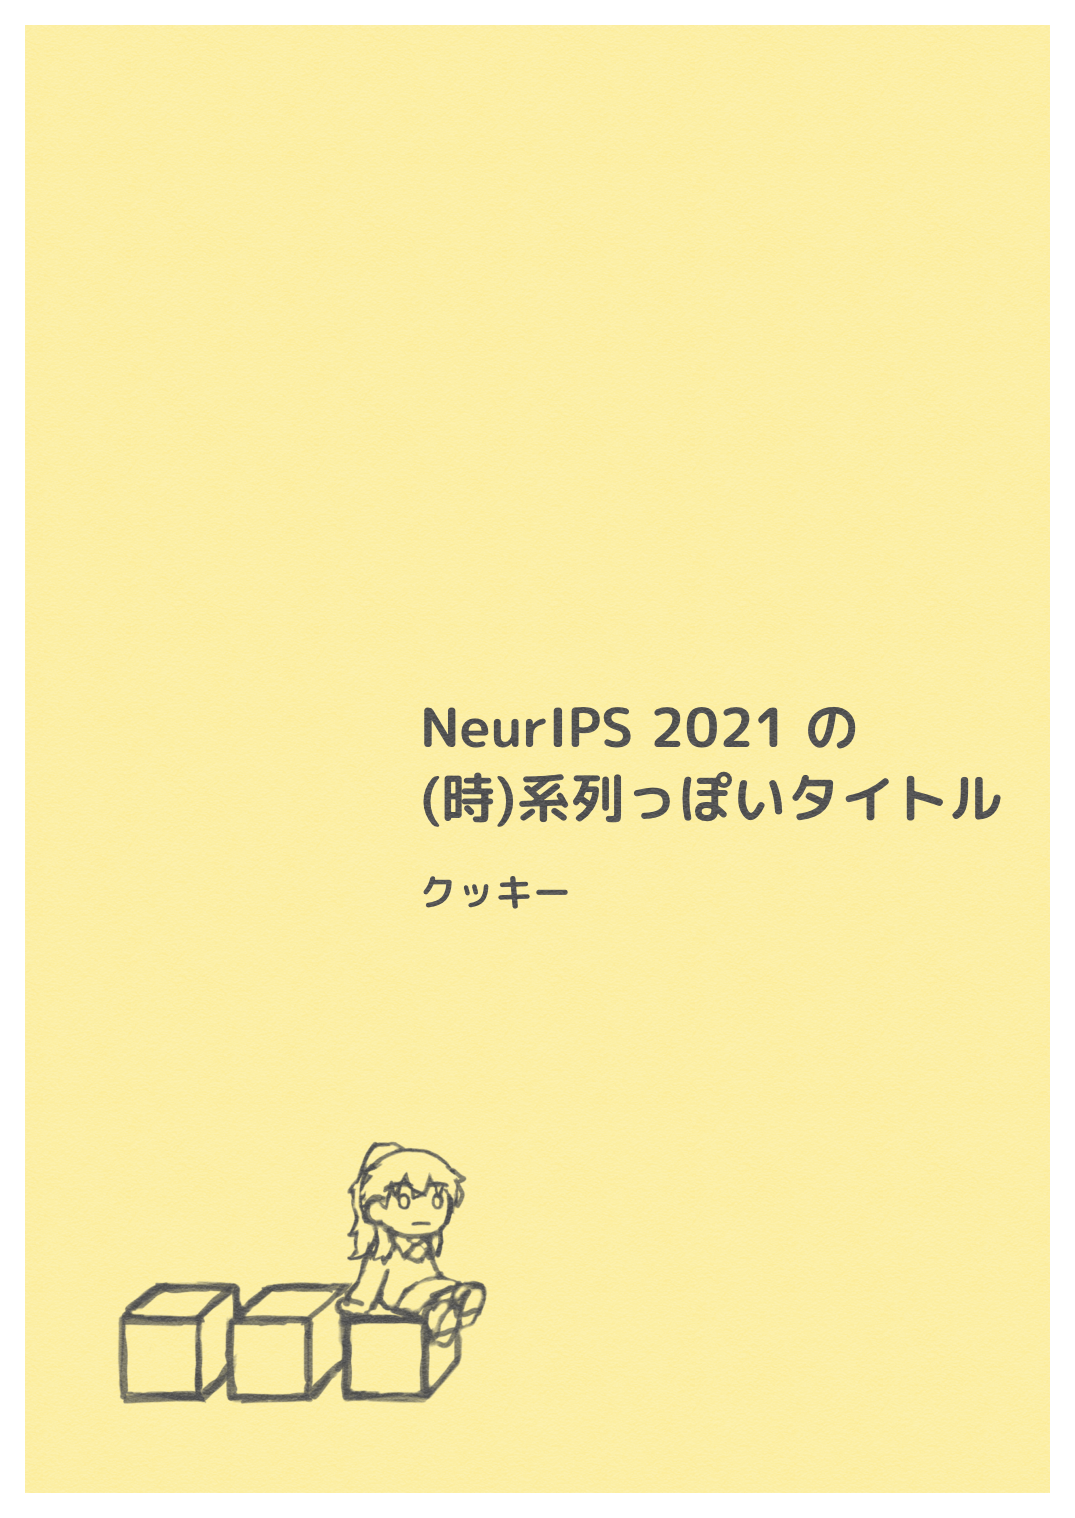
\includegraphics[width=0.99\paperwidth,height=0.99\paperheight,%
keepaspectratio]{cover.png}%
\vfill
}}}



\begin{document}

\AddToShipoutPicture*{\BackgroundPic}
\begin{titlepage}
\ 
\end{titlepage}


% 地の文の文字色をグレーに変更する
\addfontfeatures{Color=DarkGray}
\addCJKfontfeatures{Color=DarkGray}


% \part*{NeurIPS 2021 の(時)系列っぽいタイトル}

\begin{spacing}{1.0}
\tableofcontents
\end{spacing}

\section*{まえがき}
\addcontentsline{toc}{section}{まえがき}
\vspace{3pt}

お気付きの点がありましたらこの原稿のリポジトリの Issues までお願いいたします。

https://github.com/CookieBox26/notes/issues


\section*{オーバービュー}
\addcontentsline{toc}{section}{オーバービュー}
\vspace{3pt}

\begin{SERIFU}[colback=PaleIris, colbacktitle=PaleIris2]{kazusa_0.png}
NeurIPS 2021 で発表された(時)系列データを扱うモデルに関連する研究をみていきましょう。NeurIPS 2021 で発表された論文の総数は……2334本!?
\end{SERIFU}

\begin{SERIFU}[colback=PaleIris]{kazusa_1.png}
あ、あまりに多いので機械的に絞り込みましょう。タイトルに time series, sequential, rnn, recurrent, transformer, attention, state space のいずれかを含む論文は……それでも 155本……。画像認識, GAN, 強化学習系のタイトルは断腸の思いでとばしていきましょう……。
\end{SERIFU}

\begin{SERIFU}[colback=PaleIris]{kazusa_2.png}
――こうしてみると、\textbf{「セルフアテンションの計算量に対処する」}は引き続き人気(?)なテーマである一方、\textbf{「RNN を理論的に理解する」}という研究も割りにみられるように感じられます。以下は私見による整理です。
\begin{itemize}
  \item \textbf{RNN を理論的に理解する} \cite{05_Fermanian2021} \cite{18_Smith2021} \cite{21_Wang2021} \cite{22_Panigrahi2021}。
  \item RNN を工夫する。
  \begin{itemize}
    \item 訓練時に隠れ状態にノイズ添加してロバストにする \cite{06_Lim2021}。
    \item RNN 自体が時間変化できるようにする \cite{09_Zhang2021}。
  \end{itemize}

  \vspace{5pt}
  \item トランスフォーマーを理論的に理解する \cite{02_Panahi2021} \cite{16_Bricken2021}。
  \item トランスフォーマーを工夫する。
  \begin{itemize}
    \item 機械的にプレ処理(トレンド-季節性分解)をする \cite{23_Wu2021}。
    \item グリッド分割をさらにする(ビジョントランスフォーマー) \cite{17_Han2021}。
    \item \textbf{セルフアテンションの計算量に対処する} \cite{03_Chen2021} \cite{04_Ma2021} \cite{07_Dutta2021} \cite{11_Jaszczur2021} \cite{19_Chen2021} \cite{20_Zhu2021} \cite{24_Ren2021} \cite{25_Luo2021}。
    \item ヘッド間で $Q, K$ の分布を一致させる正則化をする \cite{15_Zhang2021}。
    \item トランスフォーマーのアーキテクチャ自体を再考する。
    \begin{itemize}
      \item 言語処理に適した構造を探索する \cite{08_So2021}
      \item セルフアテンションの代わりにゲート付MLPにする \cite{10_Liu2021}。
    \end{itemize}
  \end{itemize}

  \vspace{5pt}
  \item 機械的に汎用的なプレ処理(成分クラスタリング)をする \cite{14_Zhu2021}。

  \vspace{5pt}
  \item 微分方程式で記述されるシステムをニューラルネットで実現する。
  \begin{itemize}
    \item 線形時不変連続時間システムをニューラルネットで実現する \cite{01_Gu2021}。
    \item 連立微分方程式システムをベイズフィルタで解く \cite{13_Schmidt2021}。
  \end{itemize}
  
  \vspace{5pt}
  \item 系列モデルを新しい用途に活用する。
  \begin{itemize}
    \item トランスフォーマーを活用してガウス過程モデル適用時のカーネルを同定する \cite{12_Simpson2021}。
  \end{itemize}
\end{itemize}
\end{SERIFU}

\subsection*{グループ「RNNを理論的に理解する」}
\addcontentsline{toc}{subsection}{グループ「RNNを理論的に理解する」}

RNN の理論的な理解に関する論文が複数みられました。理論解析が進めばどのような系列データにどのようなニューラルアーキテクチャを用いるべきかにつながるのでしょうか?

\begin{itemize}
  \item RNN がある再生核ヒルベルト空間におけるカーネル法と捉えられることを示す \cite{05_Fermanian2021}。
  \item スイッチング線形動的システムで RNN をリバースエンジニアリングする \cite{18_Smith2021}。
  \item これまでの理論保証の制約を緩和する \cite{21_Wang2021} \cite{22_Panigrahi2021}。
\end{itemize}

\subsection*{グループ「セルフアテンションの計算量に対処する」}
\addcontentsline{toc}{subsection}{グループ「セルフアテンションの計算量に対処する」}

トランスフォーマーの計算量が取り沙汰されるのは $\mathrm{Softmax} \left( Q K ^\top / \sqrt{d} \right) \in \mathbb{R}^{N \times N}$ を求めるのに系列長 $N$ に対して $\mathcal{O}(N^2)$ の計算量がかかるためですが、$\mathcal{O}(N^2)$ を回避するために、以下のようなアプローチが取られているようです。スパース化、低ランク近似自体はこれまでも計算量削減の基本路線であったと思いますが、新たな切り口を導入しているのと、その他の独自路線アプローチもみられるのではないでしょうか。
\begin{itemize}
  \item $Q K ^\top$ の成分を間引く(スパースにする) 。
  \begin{itemize}
    \item どの成分か不要なのか自体を学習する \cite{11_Jaszczur2021}。
  \end{itemize}
  \item $Q K ^\top$ を低ランク近似する(行列分解する)。
  \begin{itemize}
    \item カーネル法の計算量削減のアプローチを応用する \cite{03_Chen2021}。
  \end{itemize}
  \item スパース化と低ランク近似を統合する \cite{19_Chen2021}。
  \vspace{5pt}
  \item $Q K ^\top$ の計算箇所でだけ入力系列を短い系列に射影する \cite{04_Ma2021}。
  \begin{itemize}
    \item 短距離依存性はそのまま計算し、長距離依存性は短い系列に射影する \cite{20_Zhu2021}。
  \end{itemize}
  \vspace{5pt}
  \item 長距離依存性については重み付き期待値に対してアテンションする \cite{24_Ren2021}。
  \vspace{5pt}
  \item 最初のセルフアテンション層では $Q K ^\top$ を計算するが、2番目以降ではそれを時間発展させる \cite{07_Dutta2021}。
  \vspace{5pt}
  \item アテンションの計算に高速フーリエ変換を応用する \cite{25_Luo2021}。
\end{itemize}

\section*{各論(未執筆)}
\addcontentsline{toc}{section}{各論(未執筆)}

\vspace{5pt}
\begin{PROP}[colback=White]{カーネル法の計算量削減のアプローチを応用する \cite{03_Chen2021}}
\textbf{原題: Skyformer: Remodel Self-Attention with Gaussian Kernel and Nystr\"om Method (Chen et al.)} 
\tcblower
トランスフォーマーはセルフアテンション層が計算量のボトルネックとなっていますが、カーネルマシンもまた内積計算がボトルネックになっている、と。そうですね、カーネル法のグラム行列のサイズもデータサイズに応じて $N \times N$ になりますものね。そこで、カーネル法で用いられる Nyström 近似を適用できるようにして適用したトランスフォーマーがスカイフォーマーであると。なぜスカイフォーマーなのか少し気になったので論文を覗いてみると \textbf{S}ymmetrization of \textbf{K}ernelized attention for N\textbf{Y}ström method なのですね…。
\end{PROP}

以下未執筆。

\addcontentsline{toc}{section}{参考文献}
\begin{thebibliography}{99}
    \bibitem{01_Gu2021} Albert Gu, Isys Johnson, Karan Goel, Khaled Saab, Tri Dao, Atri Rudra, Christopher Ré. Combining Recurrent, Convolutional, and Continuous-time Models with Linear State Space Layers. {\addfontfeatures{Color=SteelBlue}\href{https://proceedings.neurips.cc/paper/2021/hash/05546b0e38ab9175cd905eebcc6ebb76-Abstract.html}{In NeurIPS 2021}}.
    \bibitem{02_Panahi2021} Aliakbar Panahi, Seyran Saeedi, Tom Arodz. Shapeshifter: a Parameter-efficient Transformer using Factorized Reshaped Matrices. {\addfontfeatures{Color=SteelBlue}\href{https://proceedings.neurips.cc/paper/2021/hash/09def3ebbc44ff3426b28fcd88c83554-Abstract.html}{In NeurIPS 2021}}.
    \bibitem{03_Chen2021} Yifan Chen, Qi Zeng, Heng Ji, Yun Yang. Skyformer: Remodel Self-Attention with Gaussian Kernel and Nyström method. {\addfontfeatures{Color=SteelBlue}\href{https://proceedings.neurips.cc/paper/2021/hash/10a7cdd970fe135cf4f7bb55c0e3b59f-Abstract.html}{In NeurIPS 2021}}.
    \bibitem{04_Ma2021} Xuezhe Ma, Xiang Kong, Sinong Wang, Chunting Zhou, Jonathan May, Hao Ma, Luke Zettlemoyer. Luna: Linear Unified Nested Attention. {\addfontfeatures{Color=SteelBlue}\href{https://proceedings.neurips.cc/paper/2021/hash/14319d9cfc6123106878dc20b94fbaf3-Abstract.html}{In NeurIPS 2021}}.
    \bibitem{05_Fermanian2021} Adeline Fermanian, Pierre Marion, Jean-Philippe Vert, Gérard Biau. Framing RNN as a kernel method: A neural ODE approach. {\addfontfeatures{Color=SteelBlue}\href{https://proceedings.neurips.cc/paper/2021/hash/18a9042b3fc5b02fe3d57fea87d6992f-Abstract.html}{In NeurIPS 2021}}.
    \bibitem{06_Lim2021} Soon Hoe Lim, N. Benjamin Erichson, Liam Hodgkinson, Michael W. Mahoney. Noisy Recurrent Neural Networks. {\addfontfeatures{Color=SteelBlue}\href{https://proceedings.neurips.cc/paper/2021/hash/29301521774ff3cbd26652b2d5c95996-Abstract.html}{In NeurIPS 2021}}.
    \bibitem{07_Dutta2021} Subhabrata Dutta, Tanya Gautam, Soumen Chakrabarti, Tanmoy Chakraborty. Redesigning the Transformer Architecture with Insights from Multi-particle Dynamical Systems. {\addfontfeatures{Color=SteelBlue}\href{https://proceedings.neurips.cc/paper/2021/hash/2bd388f731f26312bfc0fe30da009595-Abstract.html}{In NeurIPS 2021}}.
    \bibitem{08_So2021} David So, Wojciech Mańke, Hanxiao Liu, Zihang Dai, Noam Shazeer, Quoc Le. Searching for Efficient Transformers for Language Modeling. {\addfontfeatures{Color=SteelBlue}\href{https://proceedings.neurips.cc/paper/2021/hash/2f3c6a4cd8af177f6456e7e51a916ff3-Abstract.html}{In NeurIPS 2021}}.
    \bibitem{09_Zhang2021} Aston Zhang, Yi Tay, Yikang Shen, Alvin Chan Guo Wei, SHUAI ZHANG. Self-Instantiated Recurrent Units with Dynamic Soft Recursion. {\addfontfeatures{Color=SteelBlue}\href{https://proceedings.neurips.cc/paper/2021/hash/3341f6f048384ec73a7ba2e77d2db48b-Abstract.html}{In NeurIPS 2021}}.
    \bibitem{10_Liu2021} Hanxiao Liu, Zihang Dai, David So, Quoc Le. Pay Attention to MLPs. {\addfontfeatures{Color=SteelBlue}\href{https://proceedings.neurips.cc/paper/2021/hash/4cc05b35c2f937c5bd9e7d41d3686fff-Abstract.html}{In NeurIPS 2021}}.
    \bibitem{11_Jaszczur2021} Sebastian Jaszczur, Aakanksha Chowdhery, Afroz Mohiuddin, Łukasz Kaiser, Wojciech Gajewski, Henryk Michalewski, Jonni Kanerva. Sparse is Enough in Scaling Transformers. {\addfontfeatures{Color=SteelBlue}\href{https://proceedings.neurips.cc/paper/2021/hash/51f15efdd170e6043fa02a74882f0470-Abstract.html}{In NeurIPS 2021}}.
    \bibitem{12_Simpson2021} Fergus Simpson, Ian Davies, Vidhi Lalchand, Alessandro Vullo, Nicolas Durrande, Carl Edward Rasmussen. Kernel Identification Through Transformers. {\addfontfeatures{Color=SteelBlue}\href{https://proceedings.neurips.cc/paper/2021/hash/56c3b2c6ea3a83aaeeff35eeb45d700d-Abstract.html}{In NeurIPS 2021}}.
    \bibitem{13_Schmidt2021} Jonathan Schmidt, Nicholas Krämer, Philipp Hennig. A Probabilistic State Space Model for Joint Inference from Differential Equations and Data. {\addfontfeatures{Color=SteelBlue}\href{https://proceedings.neurips.cc/paper/2021/hash/6734fa703f6633ab896eecbdfad8953a-Abstract.html}{In NeurIPS 2021}}.
    \bibitem{14_Zhu2021} Zhibo Zhu, Ziqi Liu, Ge Jin, Zhiqiang Zhang, Lei Chen, Jun Zhou, Jianyong Zhou. MixSeq: Connecting Macroscopic Time Series Forecasting with Microscopic Time Series Data. {\addfontfeatures{Color=SteelBlue}\href{https://proceedings.neurips.cc/paper/2021/hash/6b5754d737784b51ec5075c0dc437bf0-Abstract.html}{In NeurIPS 2021}}.
    \bibitem{15_Zhang2021} Shujian Zhang, Xinjie Fan, Huangjie Zheng, Korawat Tanwisuth, Mingyuan Zhou. Alignment Attention by Matching Key and Query Distributions. {\addfontfeatures{Color=SteelBlue}\href{https://proceedings.neurips.cc/paper/2021/hash/6fd6b030c6afec018415662d0db43f9d-Abstract.html}{In NeurIPS 2021}}.
    \bibitem{16_Bricken2021} Trenton Bricken, Cengiz Pehlevan. Attention Approximates Sparse Distributed Memory. {\addfontfeatures{Color=SteelBlue}\href{https://proceedings.neurips.cc/paper/2021/hash/8171ac2c5544a5cb54ac0f38bf477af4-Abstract.html}{In NeurIPS 2021}}.
    \bibitem{17_Han2021} Kai Han, An Xiao, Enhua Wu, Jianyuan Guo, Chunjing XU, Yunhe Wang. Transformer in Transformer. {\addfontfeatures{Color=SteelBlue}\href{https://proceedings.neurips.cc/paper/2021/hash/854d9fca60b4bd07f9bb215d59ef5561-Abstract.html}{In NeurIPS 2021}}.
    \bibitem{18_Smith2021} Jimmy Smith, Scott Linderman, David Sussillo. Reverse engineering recurrent neural networks with Jacobian switching linear dynamical systems. {\addfontfeatures{Color=SteelBlue}\href{https://proceedings.neurips.cc/paper/2021/hash/8b77b4b5156dc11dec152c6c71481565-Abstract.html}{In NeurIPS 2021}}.
    \bibitem{19_Chen2021} Beidi Chen, Tri Dao, Eric Winsor, Zhao Song, Atri Rudra, Christopher Ré. Scatterbrain: Unifying Sparse and Low-rank Attention. {\addfontfeatures{Color=SteelBlue}\href{https://proceedings.neurips.cc/paper/2021/hash/9185f3ec501c674c7c788464a36e7fb3-Abstract.html}{In NeurIPS 2021}}.
    \bibitem{20_Zhu2021} Chen Zhu, Wei Ping, Chaowei Xiao, Mohammad Shoeybi, Tom Goldstein, Anima Anandkumar, Bryan Catanzaro. Long-Short Transformer: Efficient Transformers for Language and Vision. {\addfontfeatures{Color=SteelBlue}\href{https://proceedings.neurips.cc/paper/2021/hash/9425be43ba92c2b4454ca7bf602efad8-Abstract.html}{In NeurIPS 2021}}.
    \bibitem{21_Wang2021} Lifu Wang, Bo Shen, Bo Hu, Xing Cao. On the Provable Generalization of Recurrent Neural Networks. {\addfontfeatures{Color=SteelBlue}\href{https://proceedings.neurips.cc/paper/2021/hash/a928731e103dfc64c0027fa84709689e-Abstract.html}{In NeurIPS 2021}}.
    \bibitem{22_Panigrahi2021} Abhishek Panigrahi, Navin Goyal. Learning and Generalization in RNNs. {\addfontfeatures{Color=SteelBlue}\href{https://proceedings.neurips.cc/paper/2021/hash/b04c387c8384ca083a71b8da516f65f6-Abstract.html}{In NeurIPS 2021}}.
    \bibitem{23_Wu2021} Haixu Wu, Jiehui Xu, Jianmin Wang, Mingsheng Long. Autoformer: Decomposition Transformers with Auto-Correlation for Long-Term Series Forecasting. {\addfontfeatures{Color=SteelBlue}\href{https://proceedings.neurips.cc/paper/2021/hash/bcc0d400288793e8bdcd7c19a8ac0c2b-Abstract.html}{In NeurIPS 2021}}.
    \bibitem{24_Ren2021} Hongyu Ren, Hanjun Dai, Zihang Dai, Mengjiao Yang, Jure Leskovec, Dale Schuurmans, Bo Dai. Combiner: Full Attention Transformer with Sparse Computation Cost. {\addfontfeatures{Color=SteelBlue}\href{https://proceedings.neurips.cc/paper/2021/hash/bd4a6d0563e0604510989eb8f9ff71f5-Abstract.html}{In NeurIPS 2021}}.
    \bibitem{25_Luo2021} Shengjie Luo, Shanda Li, Tianle Cai, Di He, Dinglan Peng, Shuxin Zheng, Guolin Ke, Liwei Wang, Tie-Yan Liu. Stable, Fast and Accurate: Kernelized Attention with Relative Positional Encoding. {\addfontfeatures{Color=SteelBlue}\href{https://proceedings.neurips.cc/paper/2021/hash/c0f168ce8900fa56e57789e2a2f2c9d0-Abstract.html}{In NeurIPS 2021}}.
\end{thebibliography}


% \vspace{5pt}
% \noindent つづかない


\end{document}
